\chapter{Introduzione}
\label{cha:intro}

I dati sono diventati una parte sempre più fondamentale della nostra vita e ancor più di quella delle aziende nell'assisterle nel processo di decision-making.
Questi dati, provenienti da molteplici fonti come: social network, online tracking, sensori di IoT, \dots, risultano in una mole enorme, non strutturati e
di conseguenza complessa da sfruttare per ricavarne informazioni rilevanti.
Proprio per questo il mondo della data integration è così importante \cite{DataIntegration}.

Possiamo definire la data integration come il problema del combinare dati provenienti da livelli diversi e fornire all'utente finale una 
visione unificata di questi\cite{dataIntegrationDef}. E' facile vedere quindi come questo concetto si adatti bene in un'azienda che utilizza vari sistemi, applicazioni 
e piattaforme, ognuna delle quali produce o raccoglie dati senza tenere conto degli altri applicativi, creando quelli che vengono definiti data silos.

Esistono approcci diversi alla data integration; quello più tradizionale è certamente quello dei data warehouse, dove tutti i dati sono combinati e memorizzati in un solo posto (tipicamente un database). 
Questo processo di "combinazione" è definito ETL (Extract, Transform, Load) e permette di rilevare e correggere inconsistenze tra i dati prima che questi vengano uniti. Permette inoltre di integrare 
tipi di dati eterogenei e visualizzarli poi come un'unica collezione complessiva.

Questa soluzione risulta complessa da utilizzare per dataset che vengono modificati frequentemente e richiedono quindi che il processo di ETL, che è molto costoso, venga re-eseguito molte volte.
Anche per questo si è quindi passati ad un paradigma basato sul \textit{loose coupling} ovvero è presente un'interfaccia sulla quale eseguire query che vengono poi mappate ed eseguite sulle sorgenti originali eliminando il 
problema dell'avere informazioni non aggiornate \cite{DataIntegrationHistory}. Questi due approcci sono descritti in figura \ref{fig:dataIntegration}.

\begin{figure}[ht]
    \centering
    \begin{minipage}{0.45\linewidth}
        \centering
        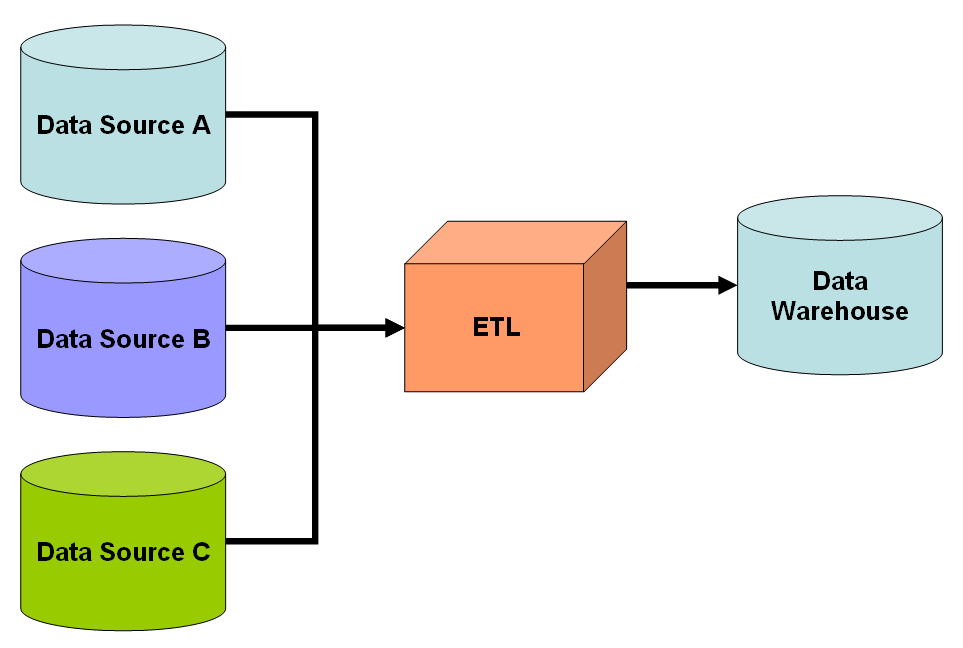
\includegraphics[width=0.9\linewidth]{Datawarehouse.png}
    \end{minipage}
    \begin{minipage}{0.45\linewidth}
        \centering
        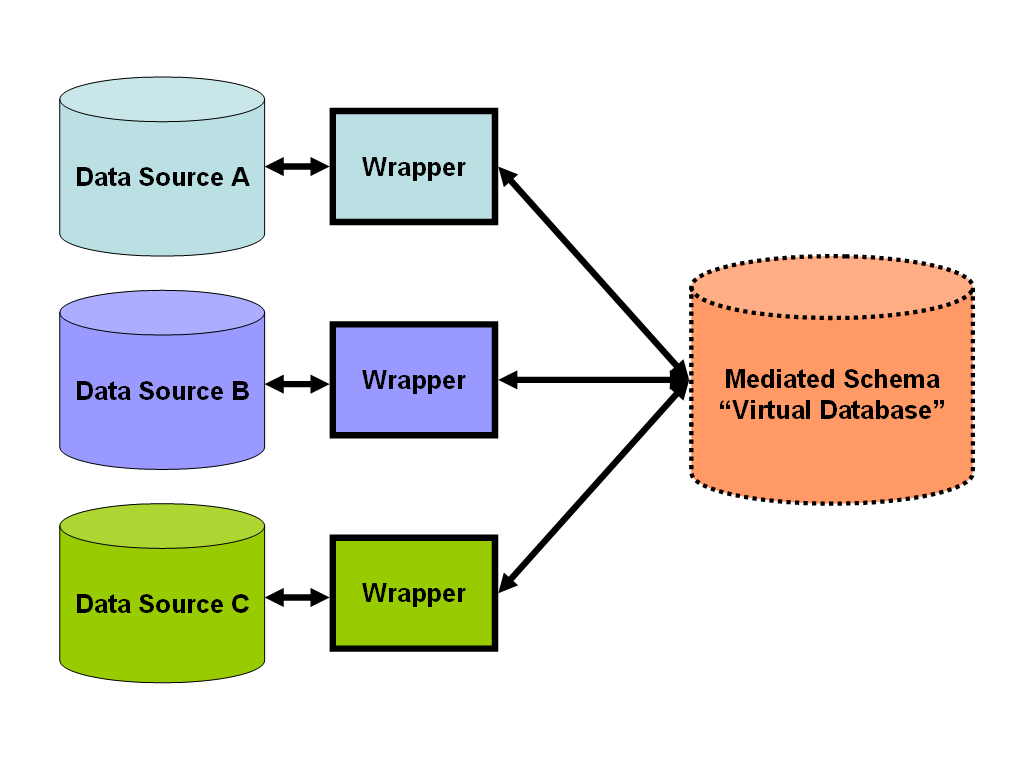
\includegraphics[width=0.9\linewidth]{Dataintegration.png}
    \end{minipage}
    \caption{Approcci alla data integration}
    \label{fig:dataIntegration}
\end{figure}
Indipendentemente dall'architettura del sistema, l'aspetto semantico risulta molto importante al fine di evitare la collisione tra termini uguali usati all'interno delle sorgenti con significati
diversi. \`E proprio da questa considerazione che nascono approcci basati su ontologie definiti come Ontology Based Data Access (OBDA). Queste soluzioni mitigano il problema appena descritto fornendo un vocabolario 
comune da utilizzare, presentano però il problema di essere complesse e di conseguenza poco fruibili da un ampio pubblico.

Lo scopo di questo elaborato è, per prima cosa, quello di descrivere i principali concetti teorici alla base delle ontologie e dei Knowledge Graph ed in particolare del Virtual Knowledge Graph system Ontop. Una volta stabilite delle
basi teoriche comuni verrà descritta l'esperienza di tirocinio da me svolta presso l'azienda Ontopic al fine di sviluppare un strumento che permetta l'interrogazione di un ontologia tramite strumenti di business intelligence 
come Tableau. In questo modo l'ontologia può essere interrogata anche da persone non esperte del campo dato che le query possono essere scritte in SQL o addirittura tramite l'interfaccia grafica fornita dagli strumenti di 
business intelligence.